% Sample document for SBGames papers
% Uses a slightly modified IEEE VGTC template in conference mode

\documentclass{vgtc}                          % final (conference style)

%% These three lines bring in essential packages: ``mathptmx'' for Type 1 
%% typefaces, ``graphicx'' for inclusion of EPS figures. and ``times''
%% for proper handling of the times font family.

\usepackage{mathptmx}
\usepackage{graphicx}
\usepackage{times}
\usepackage[utf8]{inputenc}

%% We encourage the use of mathptmx for consistent usage of times font
%% throughout the proceedings. However, if you encounter conflicts
%% with other math-related packages, you may want to disable it.

%% If you are submitting a paper to a conference for review with a double
%% blind reviewing process, please replace the value ``0'' below with your
%% OnlineID. Otherwise, you may safely leave it at ``0''.
\onlineid{0}

%% declare the category of your paper, only shown in review mode
\vgtccategory{Research}

%% Paper title.

\title{Sample Paper Title}

%% Authors are listed in up to three columns as necessary
%% with a footnote referring to a single e-mail contact.
%% Affiliations are placed after the authors, one per line
%% with superscript numbers used to link them to authors

%% Single author:
%%\author{Single author name\thanks{e-mail: email@somewhere.com}}
%%\affiliation{\scriptsize University A}

%% Multiple authors with single affiliation:
%%\author{First author\thanks{e-mail: email@somewhere.com} %
%%\and Second author %
%%\and Third author}
%%\affiliation{\scriptsize Research institute X}

%% Multiple authors with multiple affiliations:
\author{Thiago Santos Figueira$^{1}$\thanks{e-mail: email@somewhere.com} %
\and Adriano Mendes Gil$^{2}$}
\affiliation{\scriptsize $^{1}$Research institute X, Department, Country\\
$^{2}$University B, Department, Country\\
$^{3}$Company C, Department, Country}

%% Abstract section.
%% Note how the keywords must be also included in this section!
\abstract{Virtual reality applications are very sensible to delay of synchronisation between user movements and its consequences on virtual environment. A way to accelerate the logic layer execution is to move its implementation to GPU. In this work we propose an architecture of visualization based on a shader parameterized by states and game elements positioning variables. As an example of this approach, we implemented a version of classic game Snake where every visual elements are defined and drawn by shader in an unique Mesh. Simultaneously, a way to mitigate inconsistencies during data reading in virtual reality joystick \textit{Gear VR Controller} through the Kalman filter is likewise described.

\smallskip

\noindent \textbf{Keywords:} Unity, Kalman filter, shaders, virtual reality games.
} % end of abstract

%% Copyright space is enabled by default as required by guidelines.
%% It is disabled by the 'review' option or via the following command:
% \nocopyrightspace

%%%%%%%%%%%%%%%%%%%%%%%%%%%%%%%%%%%%%%%%%%%%%%%%%%%%%%%%%%%%%%%%
%%%%%%%%%%%%%%%%%%%%%% START OF THE PAPER %%%%%%%%%%%%%%%%%%%%%%
%%%%%%%%%%%%%%%%%%%%%%%%%%%%%%%%%%%%%%%%%%%%%%%%%%%%%%%%%%%%%%%%%

\begin{document}

%% The ``\maketitle'' command must be the first command after the
%% ``\begin{document}'' command. It prepares and prints the title block.

%% the only exception to this rule is the \firstsection command
\firstsection{Introduction}

\maketitle

%% do not uncomment this; use the \firstsection above
%%\section{Introduction} 
Jogos desenvolvidos na \textit{Unity} seguem uma \textit{pipeline} gráfica onde, em linhas gerais, a CPU (\textit{central processing unit}) é responsável por transmitir informações sobre elementos gráficos à GPU (\textit{graphics processing unit}) através do estágio de aplicação, onde os \textit{assets} gráficos, como modelos 3D e texturas, são carregados na VRAM (\textit{video random access memory}). Posteriormente, durante o estágio de geometria, os diferentes objetos que devem ser renderizados, seus respectivos posicionamentos e demais informes visuais relevantes são tratados pela GPU e no estágio de rasterização são convertidos em imagem\cite{akenine2008real}.

% Contextualizar a Realidade Virtual e Controladores
Em outro âmbito, os controles ou \textit{joysticks} são uma das formas de interação com dispositivos de realidade virtual, no entanto, são passíveis de ruídos devido à presença de sensores baseados em magnetômetros, originando comportamentos indesejados como \textit{jittering} durante a leitura dos dados. 

% Resumo proposta
Neste trabalho, propomos o desenvolvimento de um jogo cujas representações gráficas sejam inteiramente fundamentadas em código de GPU ao passo que as restrições lógicas concentrem-se na CPU, de maneira a atuar nos diferentes estágios da \textit{pipeline} gráfica acima apresentada. Em alusão à um clássico, o jogo \textit{Snake} será recriado para os dispositivos de realidade virtual da Samsung em uma aplicação Unity, no entanto, diferencia-se do original à medida que o jogador posiciona o objeto coletável através do controlador tendo a finalidade de fazer a serpente persegui-lo. Neste aspecto, objetivando atenuar a inconsistência do controle e melhorar o reconhecimento dos sinais de entrada, aplica-se o filtro de Kalman ao \textit{joystick}.

% * Estrutura do artigo
Analisa-se na seção \ref{sec:relatedworks} outros trabalhos que abordam sensores, uso de filtros e jogos de realidade virtual. A arquitetura proposta é detalhada na seção \ref{sec:architecture}. Apresenta-se como um jogo de realidade virtual pode ser renderizado em uma esfera invertida na seção \ref{sec:invertedsphere}. Em \ref{sec:agent}, compreende-se a movimentação da \textit{snake} e sua arquitetura de renderização. A seção \ref{sec:gearvrcontroller} explana como ocorre a aplicação do filtro de Kalman no controle para VR. Resultados são discutidos na seção \ref{sec:results}. Por fim, pautam-se as conclusões e perspectivas de trabalhos futuros na seção \ref{sec:conclusion}.

\section{Theory} \label{sec:relatedworks}

Lorem ipsum dolor sit amet, consectetuer adipiscing elit, sed diam nonummy nibh euismod tincidunt ut laoreet dolore magna aliquam erat volutpat \cite{Lorensen:1987:MCA} \cite{kindlmann:1999:SAG}. Ut wisi enim ad minim veniam, quis nostrud exercit­ation ullamcorper suscipit lobortis nisl ut aliquip ex ea commodo consequat. Duis autem vel eum iriure dolor in hendrerit in vulpu-tate velit esse molestie consequat, vel illum dolore eu feugiat nulla facilisis at vero eros et accumsan et iusto odio dignissim qui blan-dit praesent luptatum zzril delenit augue duis dolore te feugait nulla facilisi.

\subsection{Subsection One} \label{sec:architecture}

Lorem ipsum dolor sit amet, consectetuer adipiscing elit, sed diam nonummy nibh euismod tincidunt ut laoreet dolore magna aliquam erat volutpat. Ut wisi enim ad minim veniam, quis nostrud exercit­ation ullamcorper suscipit lobortis nisl ut aliquip ex ea commodo consequat. Duis autem vel eum iriure dolor in hendrerit in vulpu-tate velit esse molestie consequat, vel illum dolore eu feugiat nulla facilisis at vero eros et accumsan et iusto odio dignissim qui blan-dit praesent luptatum zzril delenit augue duis dolore te feugait nulla facilisi.

\begin{figure}[htb]
  \centering
  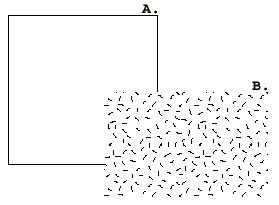
\includegraphics[width=2.76in]{figure.jpg}
  \caption{Two boxes. One filled with confetti.}
\end{figure}

\subsection{Subsection Two} \label{sec:invertedsphere}

Lorem ipsum dolor sit amet, consectetuer adipiscing elit, sed diam nonummy nibh euismod tincidunt ut laoreet dolore magna aliquam erat volutpat. Ut wisi enim ad minim veniam, quis nostrud exercit­ation ullamcorper suscipit lobortis nisl ut aliquip ex ea commodo consequat. Duis autem vel eum iriure dolor in hendrerit in vulpu-tate velit esse molestie consequat, vel illum dolore eu feugiat nulla facilisis at vero eros et accumsan et iusto odio dignissim qui blan-dit praesent luptatum zzril delenit augue duis dolore te feugait nulla facilisi.

Lorem ipsum dolor sit amet, consectetuer adipiscing elit, sed diam nonummy nibh euismod tincidunt ut laoreet dolore magna aliquam erat volutpat. Ut wisi enim ad minim veniam, quis nostrud exercit­ation ullamcorper suscipit lobortis nisl ut aliquip ex ea commodo consequat. Duis autem vel eum iriure dolor in hendrerit in vulpu-tate velit esse molestie consequat, vel illum dolore eu feugiat nulla facilisis at vero eros et accumsan et iusto odio dignissim qui blan-dit praesent luptatum zzril delenit augue duis dolore te feugait nulla facilisi.

\section{Discussion} \label{sec:agent}

Lorem ipsum dolor sit amet, consectetuer adipiscing elit, sed diam nonummy nibh euismod tincidunt ut laoreet dolore magna aliquam erat volutpat. Ut wisi enim ad minim veniam, quis nostrud exercit­ation ullamcorper suscipit lobortis nisl ut aliquip ex ea commodo consequat. Duis autem vel eum iriure dolor in hendrerit in vulpu-tate velit esse molestie consequat, vel illum dolore eu feugiat nulla facilisis at vero eros et accumsan et iusto odio dignissim qui blan-dit praesent luptatum zzril delenit augue duis dolore te feugait nulla facilisi.

\subsection{Subsection One} \label{sec:gearvrcontroller}

Lorem ipsum dolor sit amet, consectetuer adipiscing elit, sed diam nonummy nibh euismod tincidunt ut laoreet dolore magna aliquam erat volutpat. Ut wisi enim ad minim veniam, quis nostrud exercit­ation ullamcorper suscipit lobortis nisl ut aliquip ex ea commodo consequat. Duis autem vel eum iriure dolor in hendrerit in vulpu-tate velit esse molestie consequat, vel illum dolore eu feugiat nulla facilisis at vero eros et accumsan et iusto odio dignissim qui blan-dit praesent luptatum zzril delenit augue duis dolore te feugait nulla facilisi.

Lorem ipsum dolor sit amet, consectetuer adipiscing elit, sed diam nonummy nibh euismod tincidunt ut laoreet dolore magna aliquam erat volutpat. Ut wisi enim ad minim veniam, quis nostrud exercit­ation ullamcorper suscipit lobortis nisl ut aliquip 

\begin{equation}
 \sum_{j=1}^{z} j = \frac{z(z+1)}{2}
\end{equation}

ex ea commodo consequat. Duis autem vel eum iriure dolor in hendrerit in vulpu-tate velit esse molestie consequat, vel illum dolore eu feugiat nulla facilisis at vero eros et accumsan et iusto odio dignissim qui blan-dit praesent luptatum zzril delenit augue duis dolore te feugait nulla facilisi.

\subsection{Subsection Two} \label{sec:results}

Lorem ipsum dolor sit amet, consectetuer adipiscing elit, sed diam nonummy nibh euismod tincidunt ut laoreet dolore magna aliquam erat volutpat. Ut wisi enim ad minim veniam, quis nostrud exercit­ation ullamcorper suscipit lobortis nisl ut aliquip ex ea commodo consequat. Duis autem vel eum iriure dolor in hendrerit in vulpu-tate velit esse molestie consequat, vel illum dolore eu feugiat nulla facilisis at vero eros et accumsan et iusto odio dignissim qui blan-dit praesent luptatum zzril delenit augue duis dolore te feugait nulla facilisi.

\subsubsection{Subsection One} \label{sec:conclusion}

Lorem ipsum dolor sit amet, consectetuer adipiscing elit, sed diam nonummy nibh euismod tincidunt ut laoreet dolore magna aliquam erat volutpat. Ut wisi enim ad minim veniam, quis nostrud exercit­ation ullamcorper suscipit lobortis nisl ut aliquip ex ea commodo consequat. Duis autem vel eum iriure dolor in hendrerit in                                                                    vulpu-tate velit esse molestie consequat, vel illum dolore eu feugiat nulla facilisis at vero eros et accumsan et iusto odio dignissim qui blan-dit praesent luptatum zzril delenit augue duis dolore te feugait nulla facilisi.

\subsubsection{Subsection Two}

Lorem ipsum dolor sit amet, consectetuer adipiscing elit, sed diam nonummy nibh euismod tincidunt ut laoreet dolore magna aliquam erat volutpat. Ut wisi enim ad minim veniam, quis nostrud exercit­ation ullamcorper suscipit lobortis nisl ut aliquip ex ea commodo consequat. Duis autem vel eum iriure dolor in hendrerit in vulpu-tate velit esse molestie consequat, vel illum dolore eu feugiat nulla facilisis at vero eros et accumsan et iusto odio dignissim qui blan-dit praesent luptatum zzril delenit augue duis dolore te feugait nulla facilisi.

Lorem ipsum dolor sit amet, consectetuer adipiscing elit, sed diam nonummy nibh euismod tincidunt ut laoreet dolore magna aliquam erat volutpat. Ut wisi enim ad minim veniam, quis nostrud exercit­ation ullamcorper suscipit lobortis nisl ut aliquip ex ea commodo consequat. Duis autem vel eum iriure dolor in hendrerit in vulpu-tate velit esse molestie consequat, vel illum dolore eu feugiat nulla facilisis at vero eros et accumsan et iusto odio dignissim qui blan-dit praesent luptatum zzril delenit augue duis dolore te feugait nulla facilisi.

\section{Conclusion}

Lorem ipsum dolor sit amet, consectetuer adipiscing elit, sed diam nonummy nibh euismod tincidunt ut laoreet dolore magna aliquam erat volutpat. Ut wisi enim ad minim veniam, quis nostrud exercit­ation ullamcorper suscipit lobortis nisl ut aliquip ex ea commodo consequat. Duis autem vel eum iriure dolor in hendrerit in vulpu-tate velit esse molestie consequat, vel illum dolore eu feugiat nulla facilisis at vero eros et accumsan et iusto odio dignissim qui blan-dit praesent luptatum zzril delenit augue duis dolore te feugait nulla facilisi.

Lorem ipsum dolor sit amet, consectetuer adipiscing elit, sed diam nonummy nibh euismod tincidunt ut laoreet dolore magna aliquam erat volutpat. Ut wisi enim ad minim veniam, quis nostrud exercit­ation ullamcorper suscipit lobortis nisl ut aliquip ex ea commodo consequat. Duis autem vel eum iriure dolor in hendrerit in vulpu-tate velit esse molestie consequat.

\bibliographystyle{abbrv}
\bibliography{template}
\end{document}
